%-------------------------------------------------------------------------
% ds-info-S1-boucles-imbriquees.tex
%-------------------------------------------------------------------------

%-------------------------------------------------------------------------
\documentclass[11pt,a4paper]{article}
%-------------------------------------------------------------------------

%-------------------------------------------------------------------------
\input{ds-info-S1-preambule.tex}
%-------------------------------------------------------------------------

%-------------------------------------------------------------------------
\begin{document}
%-------------------------------------------------------------------------
\entete

\autoevaluation


$$\mbox{\textbf{\large Motifs géométriques}}$$


\paragraph{Questions :} 
En utilisant les instructions de la tortue \logo{}
(module \texttt{turtle}), écrire un algorithme qui dessine un motif géométrique
composé de $(n\times m)$ pavés élémentaires disposés régulièrement sur une grille
ou disposés en quinconce sur la grille.
\vspace*{3mm}

\begin{minipage}[t]{7cm}
\begin{enumerate}
\item \begin{minipage}{1.75cm}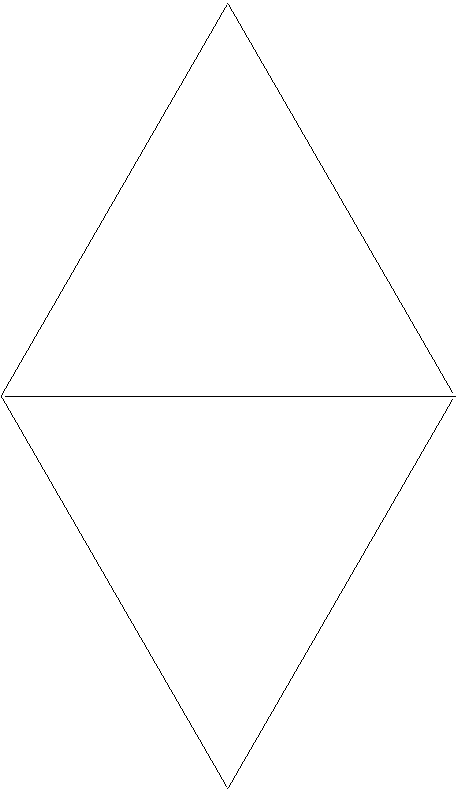
\includegraphics[height=0.75cm]{losange-2.pdf}\end{minipage} alignés
\item \begin{minipage}{1.75cm}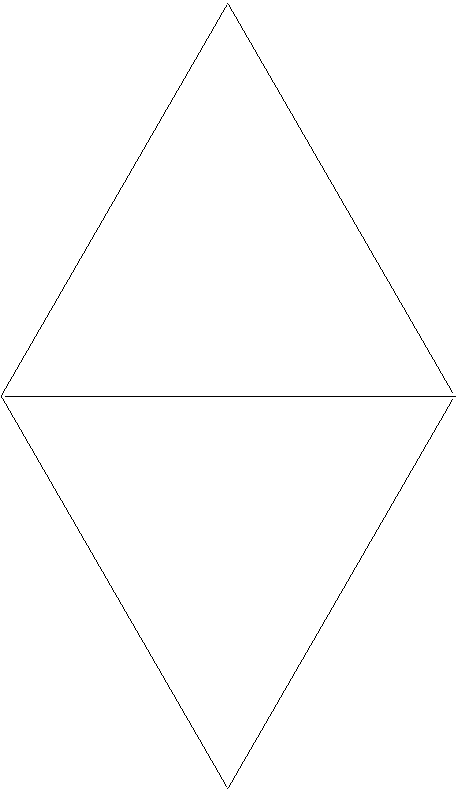
\includegraphics[height=0.75cm]{losange-2.pdf}\end{minipage} en quinconce
\item \begin{minipage}{1.75cm}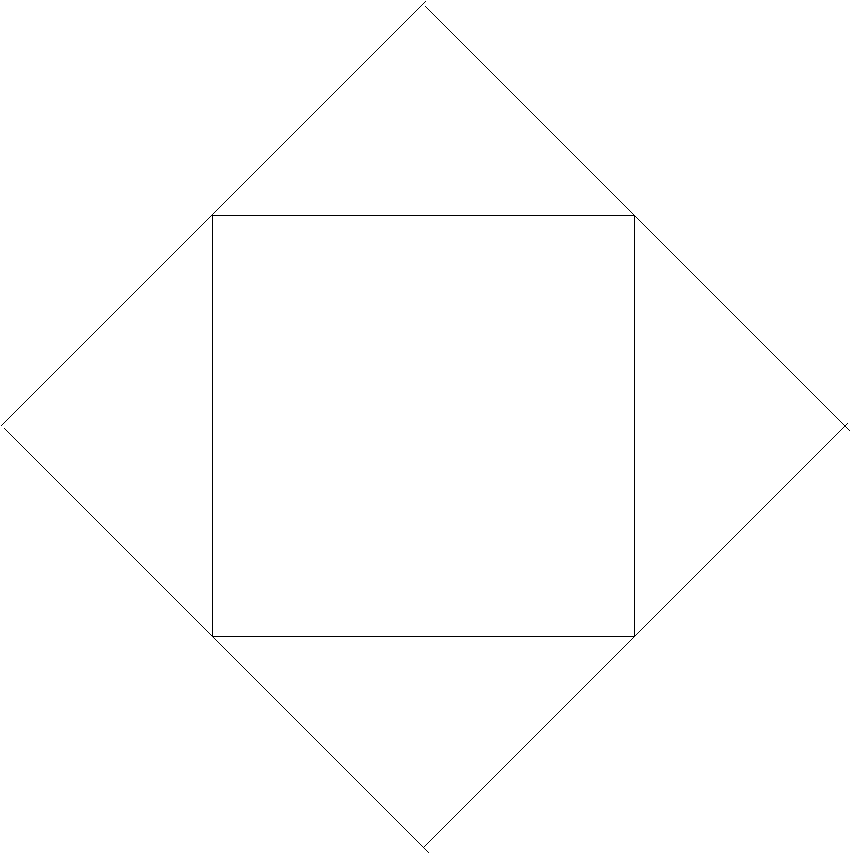
\includegraphics[height=0.75cm]{carre-2.pdf}\end{minipage} alignés
\item \begin{minipage}{1.75cm}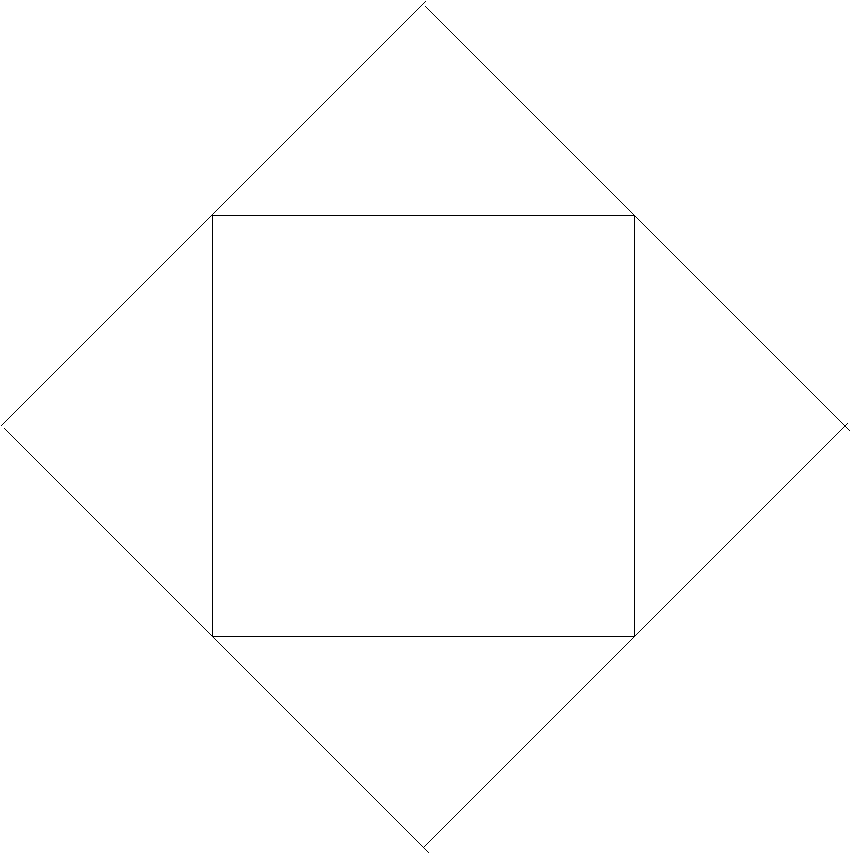
\includegraphics[height=0.75cm]{carre-2.pdf}\end{minipage} en quinconce
\item \begin{minipage}{1.75cm}\includegraphics[height=0.75cm]{etoile-2.pdf}\end{minipage} alignés
\item \begin{minipage}{1.75cm}\includegraphics[height=0.75cm]{etoile-2.pdf}\end{minipage} en quinconce
\item \begin{minipage}{1.75cm}\includegraphics[height=0.75cm]{cercle-2.pdf}\end{minipage} alignés
\item \begin{minipage}{1.75cm}\includegraphics[height=0.75cm]{cercle-2.pdf}\end{minipage} en quinconce
\item \begin{minipage}{1.75cm}\includegraphics[height=0.75cm]{hexagone-2.pdf}\end{minipage} alignés
\item \begin{minipage}{1.75cm}\includegraphics[height=0.75cm]{hexagone-2.pdf}\end{minipage} en quinconce
\item \begin{minipage}{1.75cm}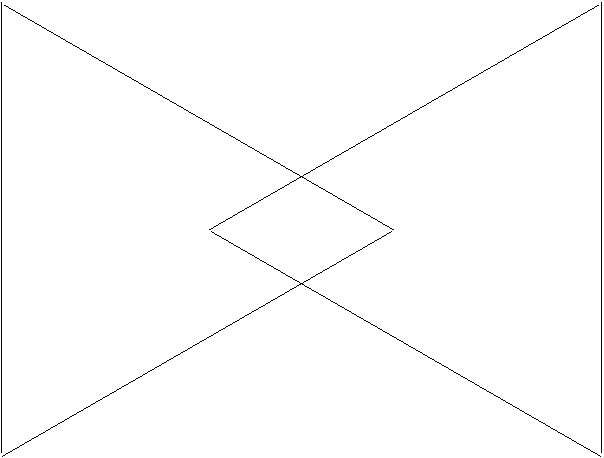
\includegraphics[height=0.75cm]{triangle-2.pdf}\end{minipage} alignés
\item \begin{minipage}{1.75cm}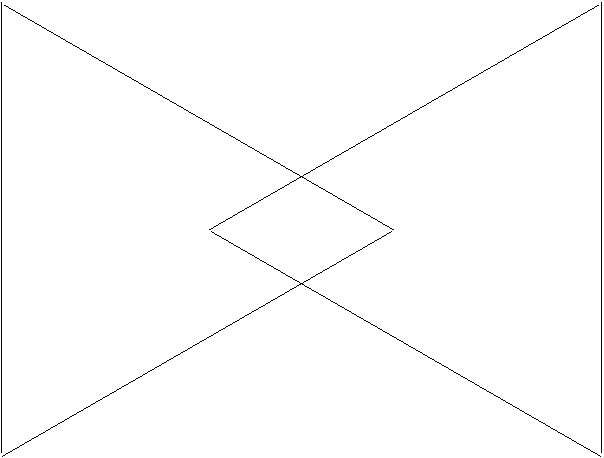
\includegraphics[height=0.75cm]{triangle-2.pdf}\end{minipage} en quinconce
\end{enumerate}
\end{minipage}
\hfill
\begin{minipage}[t]{7cm}
\begin{enumerate}\setcounter{enumi}{12}
\item \begin{minipage}{1.75cm}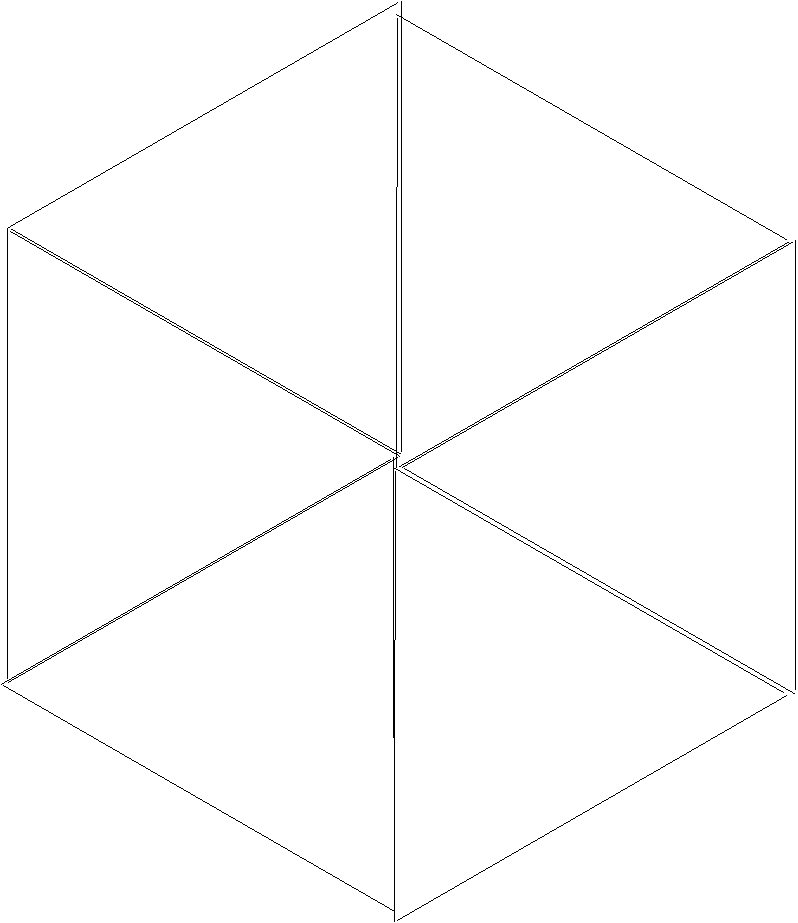
\includegraphics[height=0.75cm]{hexagone-1.pdf}\end{minipage} alignés
\item \begin{minipage}{1.75cm}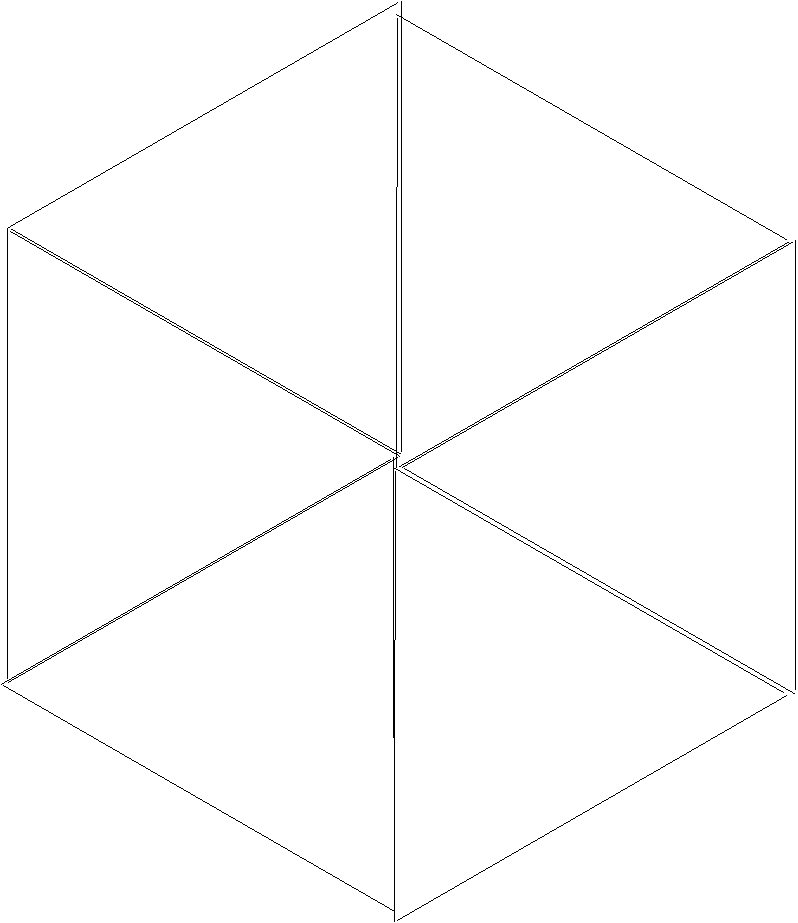
\includegraphics[height=0.75cm]{hexagone-1.pdf}\end{minipage} en quinconce
\item \begin{minipage}{1.75cm}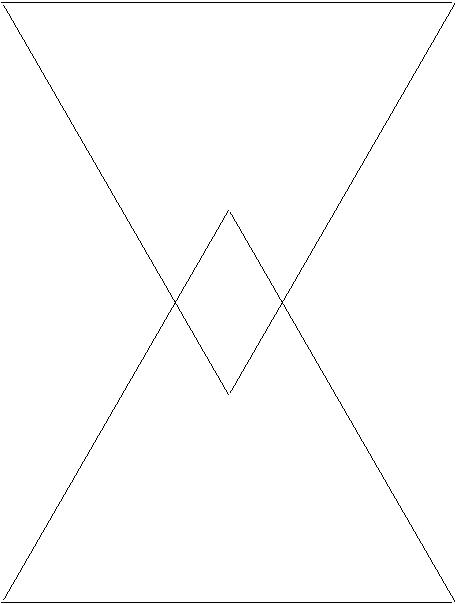
\includegraphics[height=0.75cm]{triangle-1.pdf}\end{minipage} alignés
\item \begin{minipage}{1.75cm}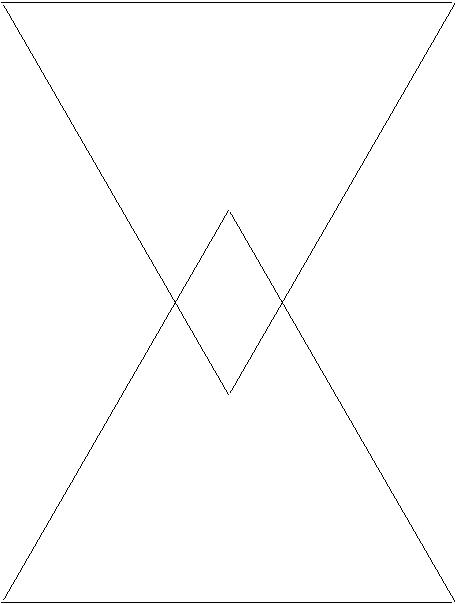
\includegraphics[height=0.75cm]{triangle-1.pdf}\end{minipage} en quinconce
\item \begin{minipage}{1.75cm}\includegraphics[height=0.75cm]{losange-1.pdf}\end{minipage} alignés
\item \begin{minipage}{1.75cm}\includegraphics[height=0.75cm]{losange-1.pdf}\end{minipage} en quinconce
\item \begin{minipage}{1.75cm}\includegraphics[height=0.75cm]{carre-1.pdf}\end{minipage} alignés
\item \begin{minipage}{1.75cm}\includegraphics[height=0.75cm]{carre-1.pdf}\end{minipage} en quinconce
\item \begin{minipage}{1.75cm}\includegraphics[height=0.75cm]{etoile-1.pdf}\end{minipage} alignés
\item \begin{minipage}{1.75cm}\includegraphics[height=0.75cm]{etoile-1.pdf}\end{minipage} en quinconce
\item \begin{minipage}{1.75cm}\includegraphics[height=0.75cm]{cercle-1.pdf}\end{minipage} alignés
\item \begin{minipage}{1.75cm}\includegraphics[height=0.75cm]{cercle-1.pdf}\end{minipage} en quinconce
\end{enumerate}
\end{minipage}
%-------------------------------------------------------------------------
\null\vfill

$$\reponse$$
%-------------------------------------------------------------------------
\paragraph{Réponse :}\mbox{}

\noindent\framebox[\textwidth]{$\rule{0cm}{0.96\textheight}$}



%-------------------------------------------------------------------------
\end{document}
%-------------------------------------------------------------------------
